\documentclass[aspectratio=1610]{beamer}

\usetheme{KTH}
\useinnertheme[shadow]{rounded}
\setbeamercolor{block title example}{fg=black,bg=lightgray}
\setbeamercolor{block body example}{fg=white,bg=gray}
\setbeamercolor{block body}{fg=white,bg=blue!60}

% remove this if using XeLaTeX or LuaLaTeX
\usepackage[utf8]{inputenc}
\usepackage{graphics}
\usepackage{graphicx}
\usepackage{booktabs}
\usepackage{ragged2e}
\usepackage{lipsum}
\usepackage{minted}
\usepackage{tikz}
\usepackage{array}
\usepackage{algorithm,algorithmicx}
\usepackage{algpseudocode}
\usepackage{amsmath,amsfonts,amssymb}
\usepackage[export]{adjustbox}
\setbeamertemplate{caption}[numbered]


\begin{document}

%------------------------------------------------
\begin{frame}[noframenumbering,plain]

  \vspace{0.02\textheight}

\begin{columns}[]
\column{37em}
\Large{\centerline{\usebeamercolor[fg]{title}Estimation of the Mass of a Manipulator Payload in Motion}}

\Large{\centerline{\usebeamercolor[fg]{title} by Means of a FT Sensor}}

\vspace{0.1\textheight}

\small{\centerline{François \textsc{Le Rall}}}
\scriptsize{\centerline{\tt francois@nomagic.ai}}
\scriptsize{\centerline{}}
\end{columns}
\end{frame}

%------------------------------------------------
\usebackgroundtemplate{\vbox{\null\vspace{3mm}
  \hspace{3mm}\pgfuseimage{kthlogosmall}\par
  \vspace{72mm}\hbox{\hspace{-75mm}\pgfuseimage{kthplatta}}}}

%------------------------------------------------
% \begin{frame}
% \frametitle{\textit{Pick-and-place} at its very beginning}
%
% \begin{figure}
% \centering
%   \begin{minipage}{.49\textwidth}
%   \centering
%   \includegraphics[width=.9\linewidth]{figs/kid.jpg}
%   \caption{Kid experiencing \textit{P\&P}}
%   \end{minipage}
%   \begin{minipage}{.49\textwidth}
%   \centering
%   \includegraphics[width=.9\linewidth]{figs/unimation.jpg}
%   \caption{\footnotesize \textsc{Unimate}: first \textit{P\&P} robot (1954)}
%   \end{minipage}
% \end{figure}
% \end{frame}
%
% %------------------------------------------------
%
% \begin{frame}
% \frametitle{Automation of industrial tasks}
% \begin{columns}
% \begin{column}{0.5\textwidth}
%   \begin{itemize}\itemsep1em
%     \justifying
%     \item \textcolor{Ocean}{Fulfill} orders
%     \item \textcolor{Ocean}{Place} electronic components on Printed Circuit Board
%     \item \textcolor{Ocean}{Assemble} products
%     \item \textcolor{Ocean}{Load} and \textcolor{Ocean}{unload} manufacturing devices
%   \end{itemize}
% \end{column}
% \begin{column}{0.5\textwidth}  %%<--- here
%   \begin{figure}
%     \centering
%     \includegraphics[width=\linewidth]{figs/maria.jpg}
%     \caption{\textit{E-commerce} picking robot}
%   \end{figure}
% \end{column}
% \end{columns}
%
% \end{frame}
%
% %------------------------------------------------
% \begin{frame}
% \frametitle{Industrial challenges}
% \begin{columns}
% \column{37em}
% \begin{itemize}\itemsep1em
%   \justifying
%   \item Handle a wide \textcolor{Ocean}{diversity of objects}
%   \item Pick \textcolor{Ocean}{unknown items} at \textcolor{Ocean}{unknown positions}
%   \item Execute tasks \textcolor{Ocean}{faster and faster}
%   \item \textcolor{Ocean}{Minimize hard failures} requiring human intervention
%   \item Perform \textcolor{Ocean}{object recognition or pose estimation} while running the \textit{P\&P} tasks
%   \item \textcolor{Ocean}{Adapt trajectories} to the item handled
% \end{itemize}
% \end{columns}
% \end{frame}
%
%
% %------------------------------------------------
% \begin{frame}
% \frametitle{Motivations behind mass estimation}
% \begin{columns}
% \column{37em}
% \begin{itemize}\itemsep1em
%   \justifying
%   \item Feature for \textcolor{Ocean}{item recognition}
%   \item Parameter for higly-dynamic \textcolor{Ocean}{force-guided} or \textcolor{Ocean}{force-guarded motion}
%   \item Attribute to detect \textcolor{Ocean}{hard failures}:
%   \begin{itemize}\itemsep1em
%     \justifying
%     \item two items grasped instead of one
%     \item item lost during motion
%     \item item hit due to oversize
%   \end{itemize}
%   \item Valuable parameter for \textcolor{Ocean}{item pose estimation}
% \end{itemize}
% \end{columns}
% \end{frame}
%
% %------------------------------------------------
%
% \begin{frame}
% \frametitle{Hardware setup}
% \begin{columns}
% \begin{column}{0.5\textwidth}
%   \begin{itemize}\itemsep1em
%     \justifying
%     \item UR10e robotic manipulator from \textsc{Universal Robot}
%     \item Pneumatic vacuum gripper
%     \item Force/Torque sensor mounted on the last wrist
%     \item \textit{Pick-and-place} tasks:
%     \begin{itemize}\itemsep0.0em
%       \justifying
%       \item tote to tote
%       \item cart to box
%     \end{itemize}
%   \end{itemize}
% \end{column}
% \begin{column}{0.5\textwidth}  %%<--- here
%   \begin{figure}
%     \centering
%     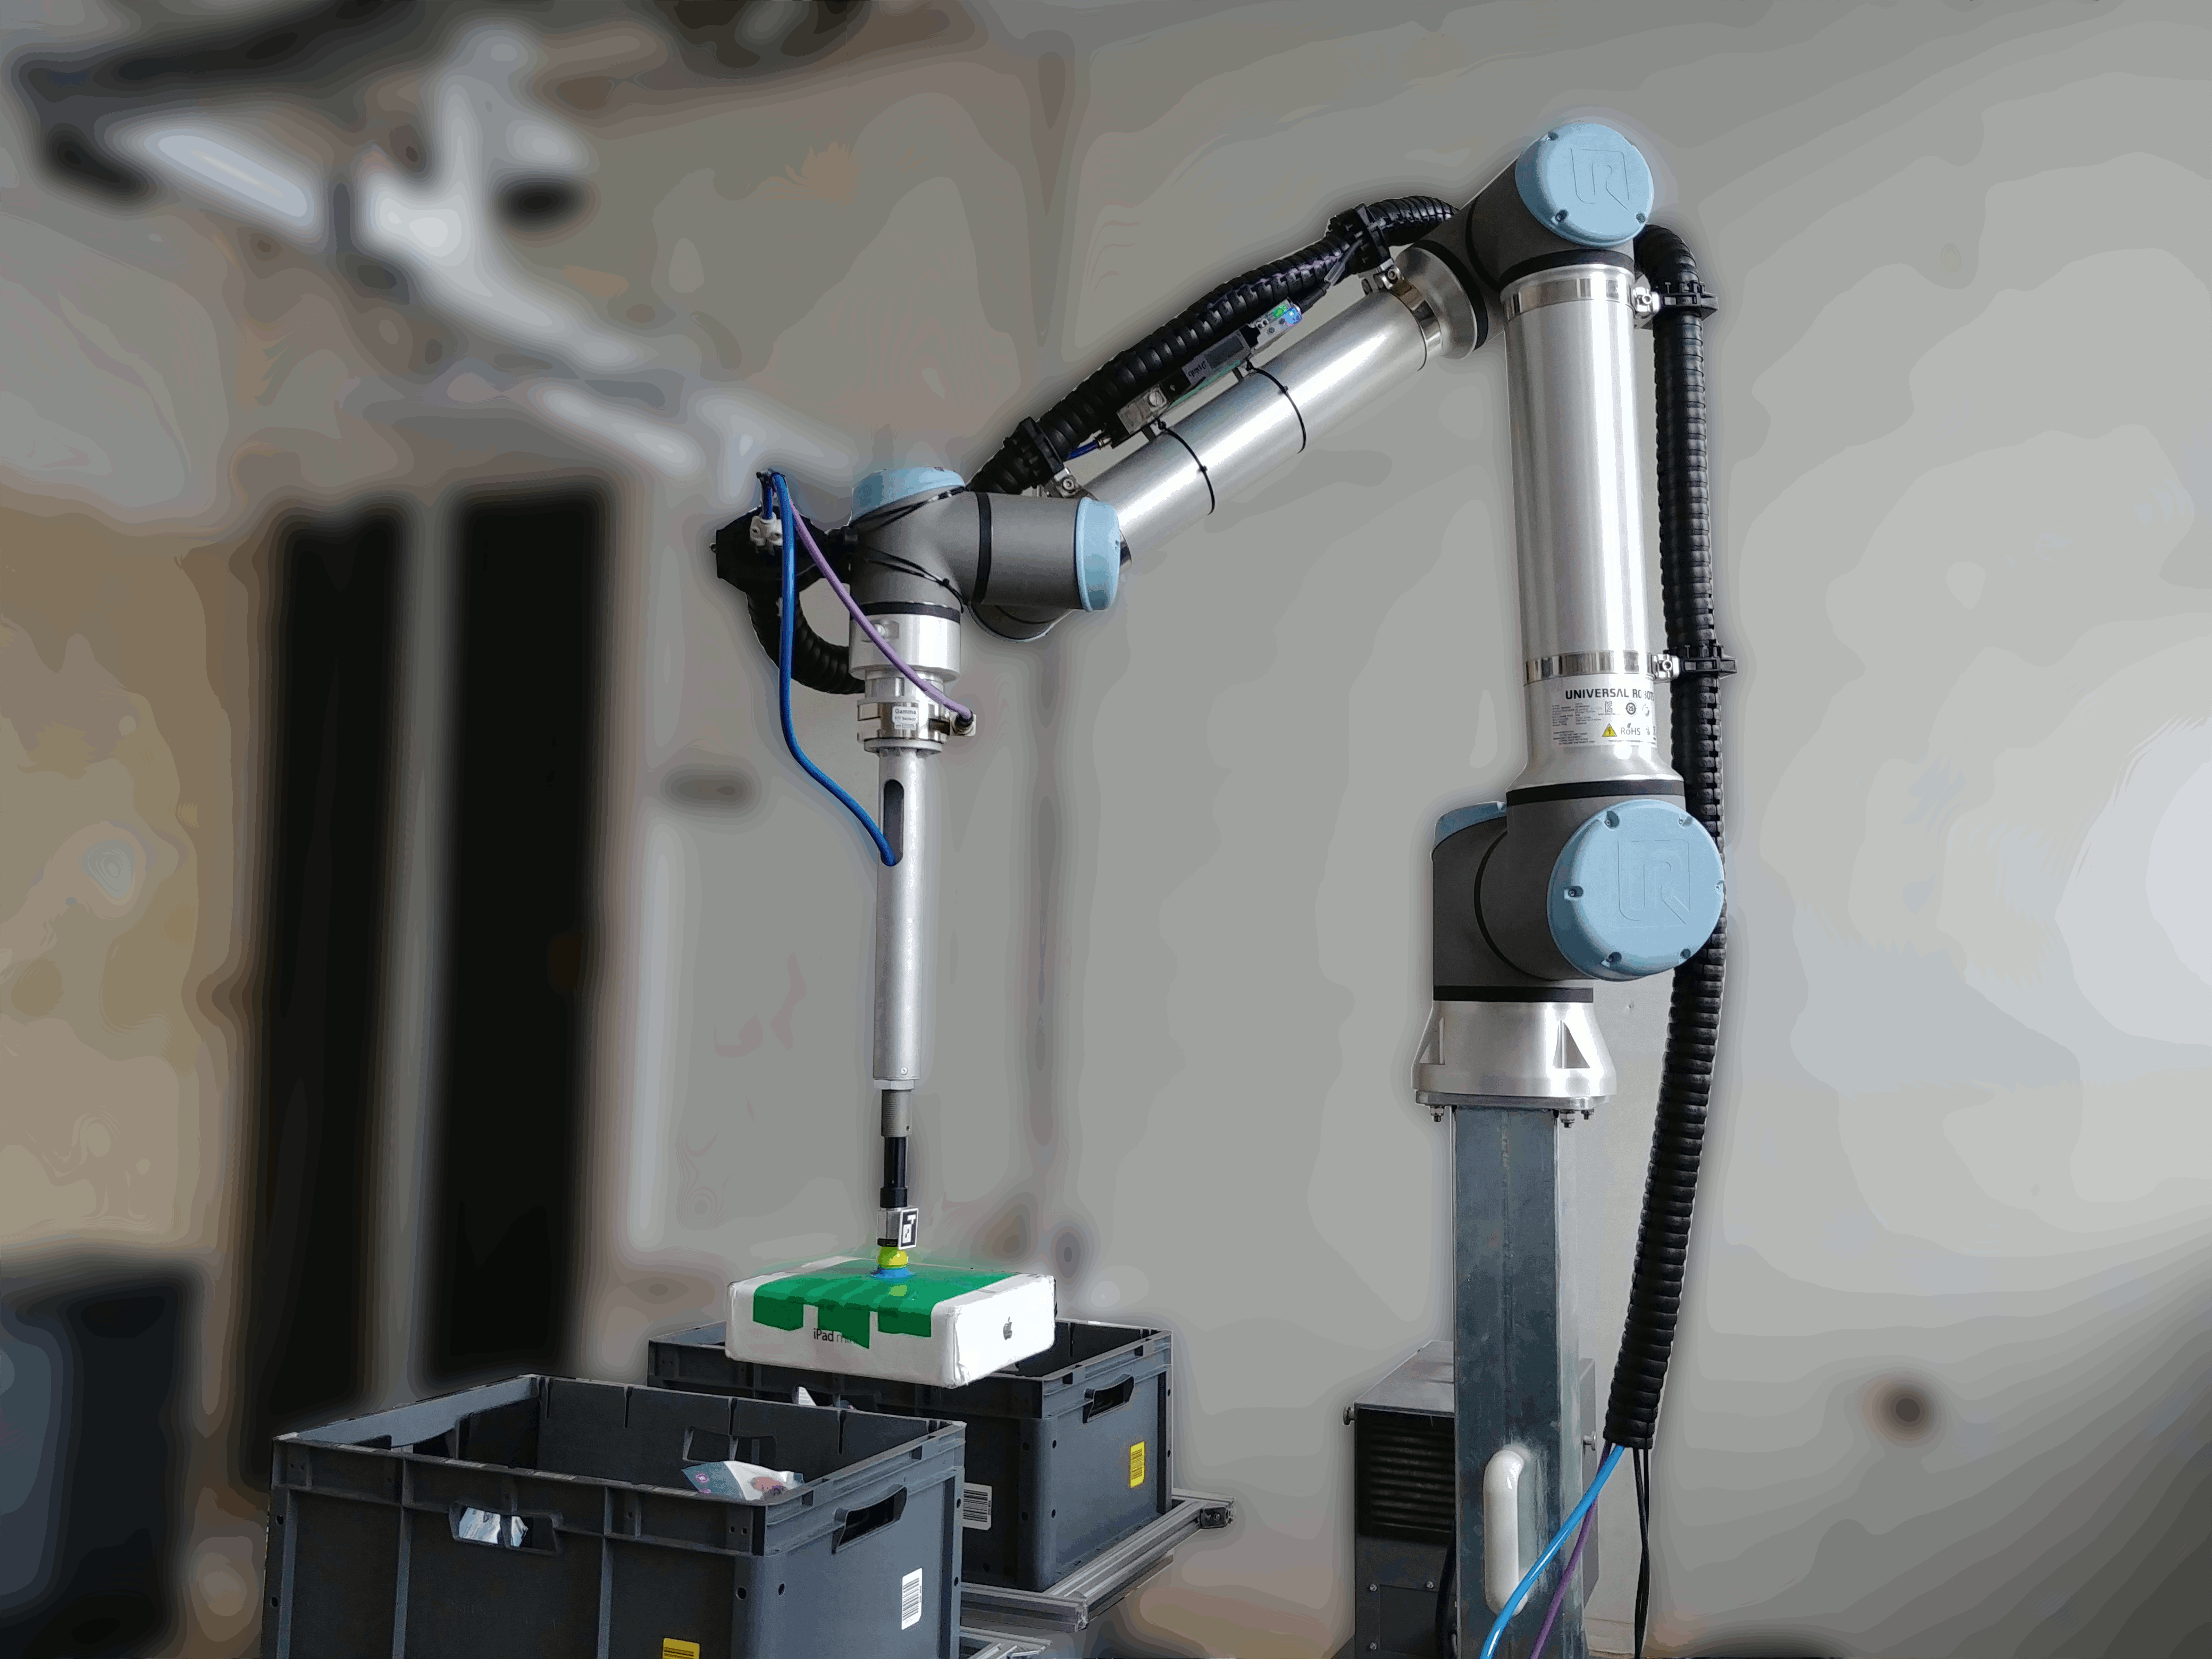
\includegraphics[width=\linewidth]{figs/picture_of_ur_indexed.png}
%     \caption{UR10e robotic arm}
%   \end{figure}
% \end{column}
% \end{columns}
%
% \end{frame}

%------------------------------------------------
\begin{frame}
\frametitle{Project background – Literature review}
\begin{columns}
\column{37em}
\begin{itemize}\itemsep1em
  \justifying
  \item \textcolor{darkred}{80-90's} Estimation of the inertial parameters of the links of the robotic manipulator
  \item \textcolor{darkred}{00-10's} Estimation of the inertial parameters of the payload
\end{itemize}


\setbeamertemplate{block begin}[default]
\setbeamertemplate{block end}[default]

\begin{block}{}
Estimate all inertial parameters to predict the mass
\end{block}



\end{columns}
\end{frame}
%
% %------------------------------------------------
%
% \begin{frame}
% \frametitle{Suction cup gripper}
% \begin{columns}
% \begin{column}{0.5\textwidth}
%   \begin{itemize}\itemsep1em
%     \justifying
%     \item \textcolor{TextGreen}{Simple integration logic}
%     \item \textcolor{TextGreen}{Versatile ability to grasp objects}
%     \item \textcolor{TextGreen}{Good grip on large range of textures}
%     \item \textcolor{darkred}{Risk of item lost}
%     \item \textcolor{darkred}{Oscillation during the motion}
%     \item \textcolor{darkred}{No existing mechanical model of the link between the tool and the item}
%   \end{itemize}
% \end{column}
% \begin{column}{0.5\textwidth}  %%<--- here
%   \begin{figure}
%     \centering
%     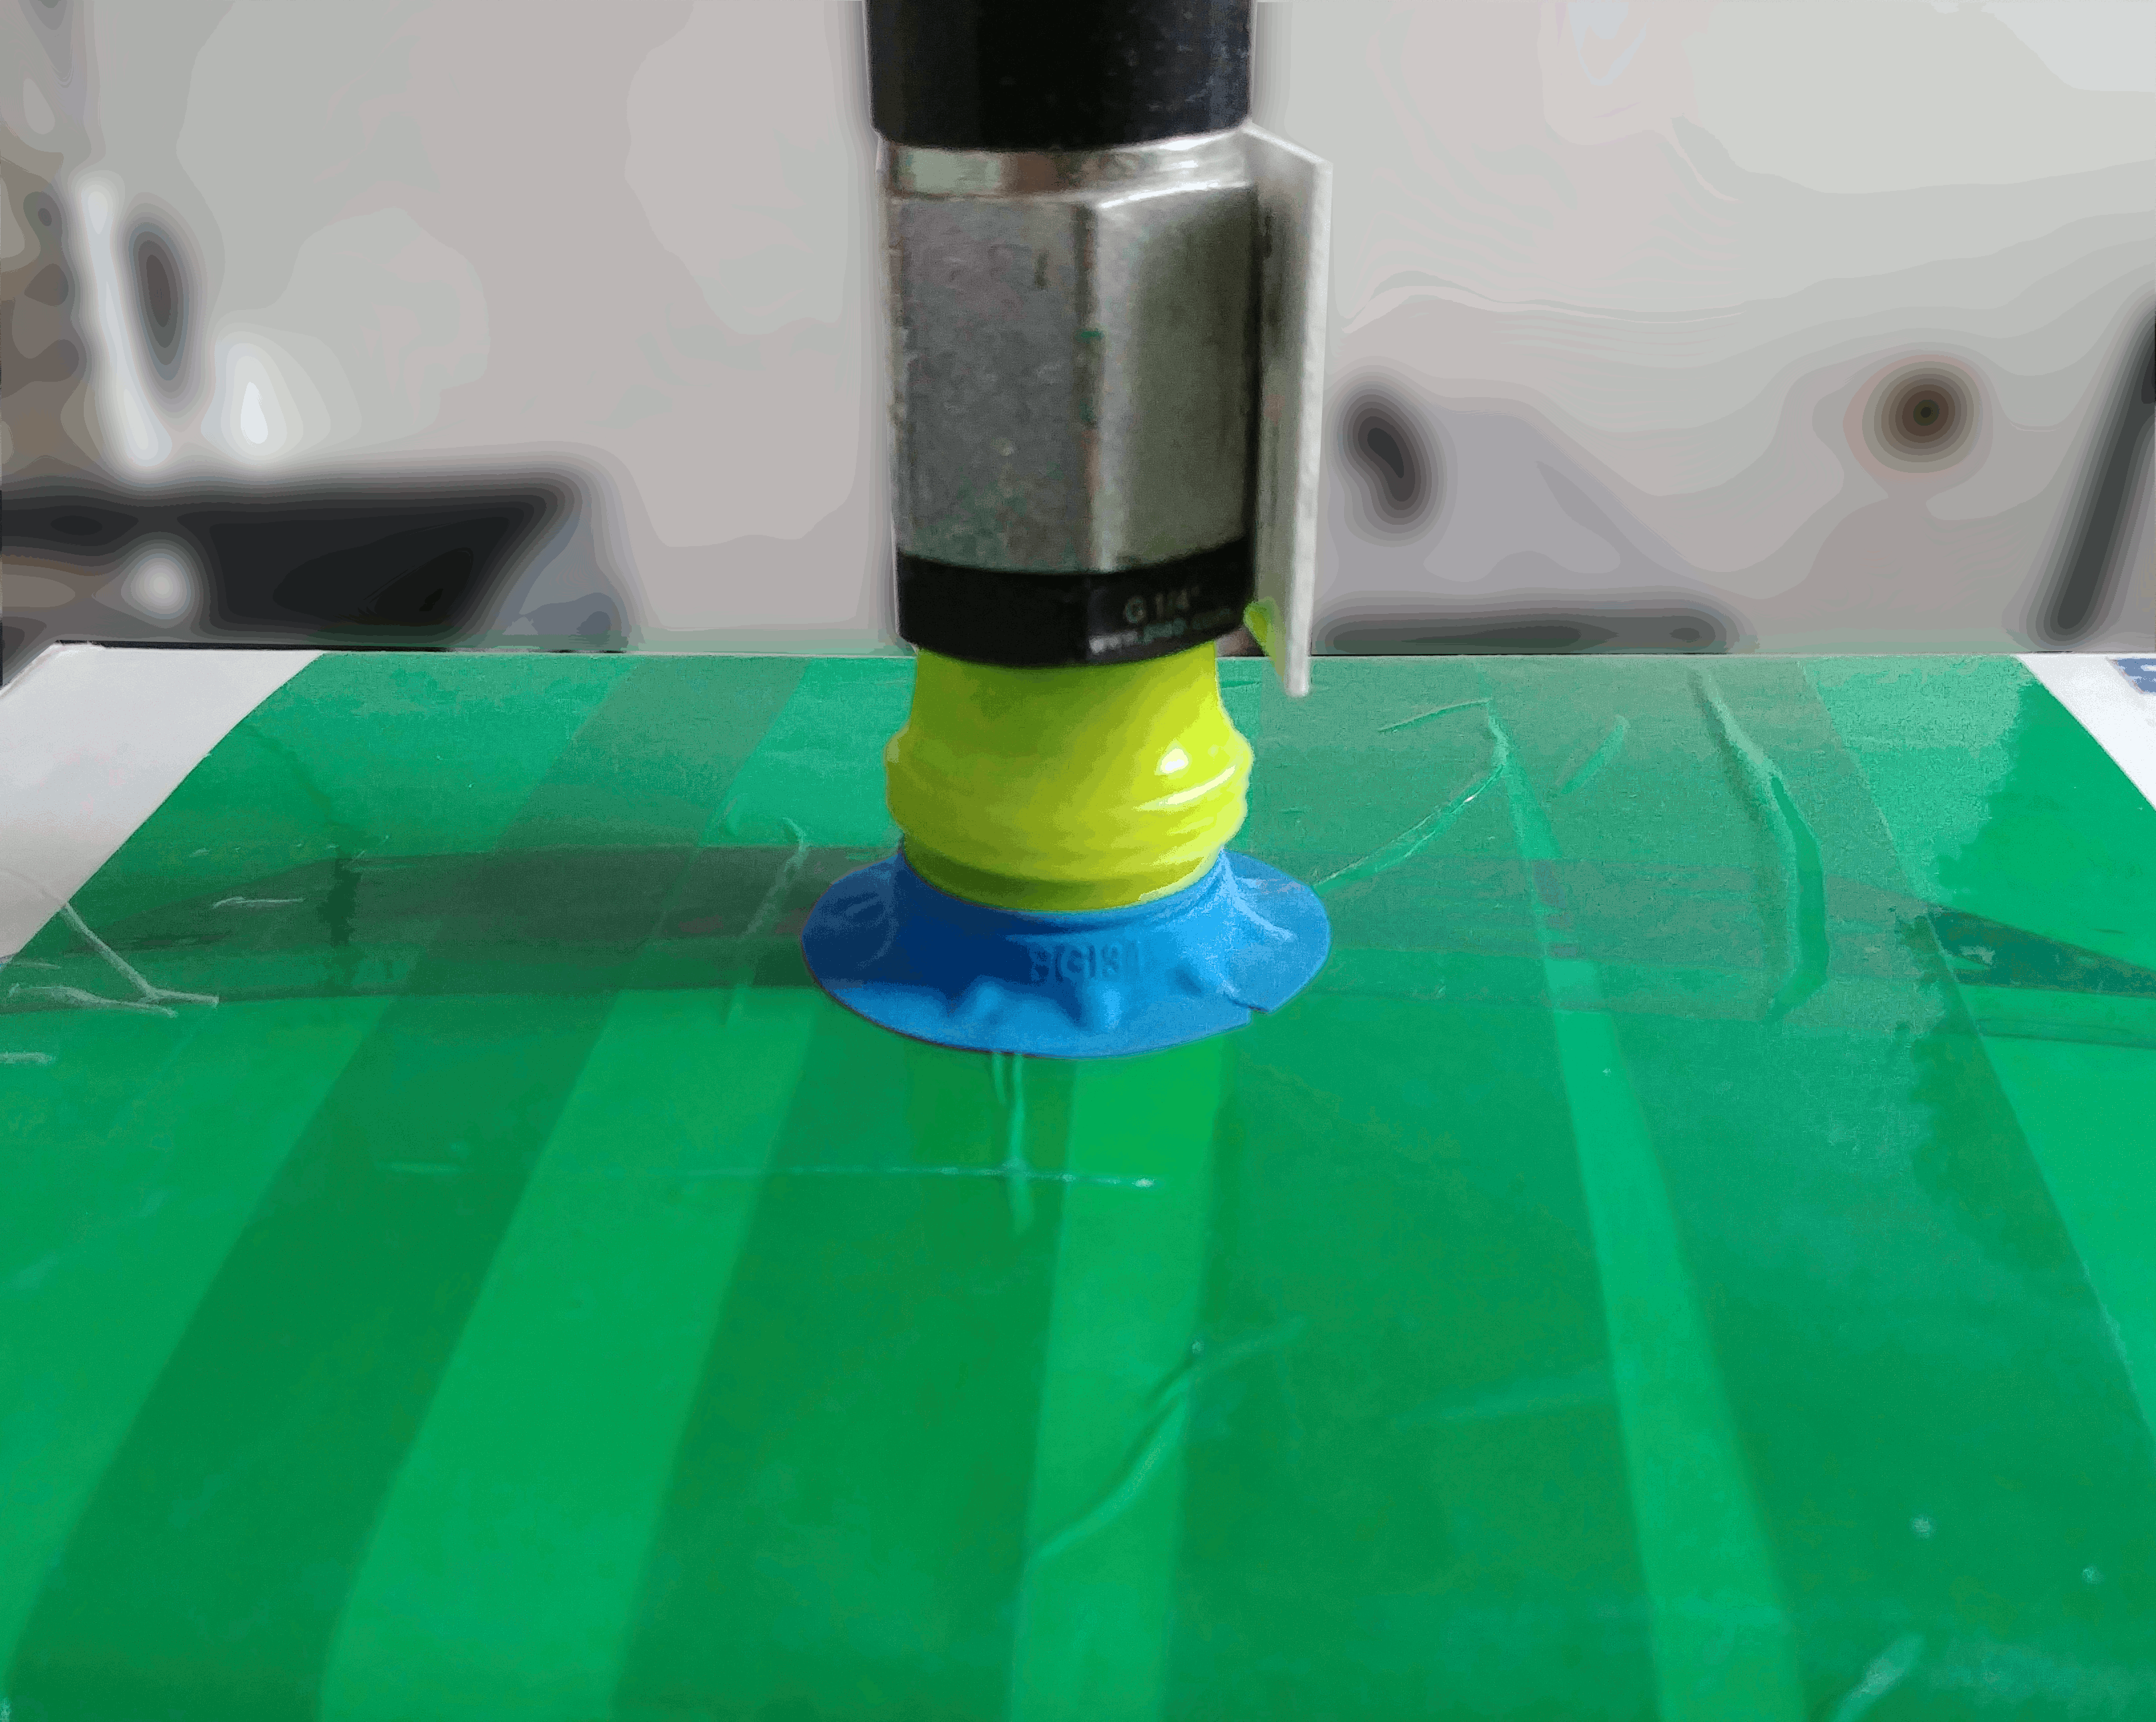
\includegraphics[scale=0.055]{figs/suction_loaded_indexed.png}
%     \caption{Suction cup gripper}
%   \end{figure}
% \end{column}
% \end{columns}
%
% \end{frame}
%
%
% %------------------------------------------------
% \begin{frame}
% \frametitle{Framework for the estimation of the mass}
% \begin{columns}
% \column{37em}
% \begin{figure}
%   \centering
%   \includegraphics[width=\linewidth]{figs/olinpe.pdf}
%   \caption{Overview of the approach}
% \end{figure}\end{columns}
% \end{frame}
%
% %------------------------------------------------
% \begin{frame}
% \begin{columns}
% \column{37em}
% \vspace{1cm}
% \Huge{\centerline{\usebeamercolor[fg]{title}Thanks!}}
% \end{columns}
% \end{frame}
%
\end{document}
% darkred TextGreen Ocean
